\documentclass{standalone}
\usepackage{tikz}
\usetikzlibrary{automata, positioning, arrows}

\begin{document}
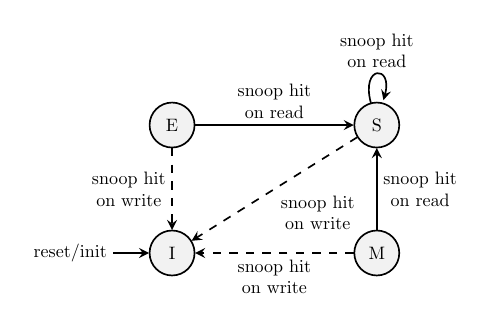
\begin{tikzpicture}[node distance=2.5cm,initial text={reset/init}]
\tikzstyle{every node}=[scale=0.65]
\tikzstyle{every state}=[semithick, fill=gray!10]
\tikzstyle{every edge}=[draw,->,>=stealth,auto,semithick]

\node[state, initial] (I) {I};
\node[state,above of=I] (E) {E};
\node[state,right of=I,node distance=4cm] (M) {M};
\node[state,right of=E,node distance=4cm] (S) {S};

\draw (M) edge[dashed] node[align=center] {snoop hit\\on write} (I)
        edge node[align=center,right] {snoop hit\\on read} (S);
\draw (S) edge[dashed] node[align=center] {snoop hit\\on write} (I)
        edge[loop above] node[align=center] {snoop hit\\on read} (S);
\draw (E) edge[dashed] node[align=center,left] {snoop hit\\on write} (I)
        edge node[align=center] {snoop hit\\on read} (S);
\end{tikzpicture}
\end{document}
